\chapter{Functional Methods in QFT}\label{chap:methods}
This chapter introduces a treatment of quantum field theory using functional methods. The main goal is to become familiar with the concepts and the formal and diagrammatic notation used throughout this work and to derive the Dyson-Schwinger Equations \cite{Dyson1949, Schwinger1951} in a simple scalar theory setting. To conclude this formal introduction to the subject, we will introduce the K\"all\'{e}n-Lehmann spectral representation for correlation functions \cite{Kallen1952, Lehmann1954}. Concerning notational conventions and for most parts of the presented derivations we closely follow \cite{NPgaugeLecture}.

\section{Generating Functionals and Dyson-Schwinger Equations}
Consider a theory setting of $N$ real scalar fields $\varphi_a(x), a \in \{1,\dots,N\}$ in $d$-dimensional Euclidean space described by the action functional
\begin{equation}
S[\varphi]=\int_{x} \frac{1}{2}\left(\partial_{\mu} \varphi\right)^{2}+\frac{m^{2}}{2} \varphi^{2}+\frac{\lambda_4}{4 !} \varphi^{4}, \label{eqn:phi4_action}
\end{equation}
and the corresponding partition sum in presence of external sources $J_a(x)$ 
\begin{align}
	Z[J] = \frac{1}{\mathcal{N}} \int \D\varphi \operatorname{e}^{-S[\varphi] + J\cdot\varphi},
	\label{eqn:partition}
\end{align}
with some normalization constant $\mathcal{N}$ and the usual path integral measure 
\begin{equation}
\mathcal{D}\varphi = \prod_{a=1}^{N} \dd \varphi_a.
\end{equation} 
In this notation the scalar product sums over field components and integrates over all space,
\begin{align}
	J\cdot\varphi = \int_x J_a(x) \ \varphi_a(x) = \int_p \tilde{J}_a(p) \ \tilde{\varphi}_a(p),
\end{align}
with the integral conventions
\begin{align}
\int_x = \int_{\mathbb{R}^d} \dd^d x \qquad \text{and} \qquad \int_p = \int_{\mathbb{R}^d} \frac{\dd^d p}{(2\pi)^d}.	
\end{align}

The partition sum $Z[J]$ is called a \textit{generating functional}. Field expectation values are computed via functional derivatives of the partition sum,
\begin{align}
	\phi := \cf{\varphi} = \eval{\frac{1}{Z}\frac{\delta Z}{\delta J}}_{J=0} = \int \D\varphi \ \varphi \ \operatorname{e}^{-S[\varphi] + J\cdot\varphi}.
\end{align}
This is generalized straightforwardly to higher order correlation functions, that are obtained as the $n$-th moments of $Z[J]$,
\begin{align}
\cf{\varphi(x_1) \cdots \varphi(x_n)} := \cf{\varphi^n} = \frac{1}{Z}\eval{\frac{\delta^n Z}{\delta^n J}}_{J=0} = \int \D\varphi \ \underbrace{\varphi_1 \cdots \varphi_n}_{=: \ \varphi^n} \ \operatorname{e}^{-S[\varphi] + J\cdot\varphi}.
\end{align}

\begin{figure}[t]
\centering
	\begin{align*}
\cf{\varphi^4} \hspace{1em}= \hspace{-1em}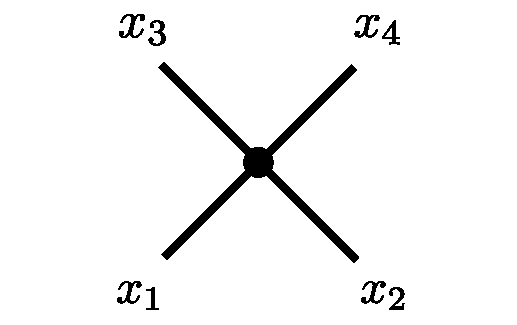
\includegraphics[scale=0.45, valign=c]{figs/diagrams/correlations/connected_01} \hspace{-1em}+ \hspace{-1em}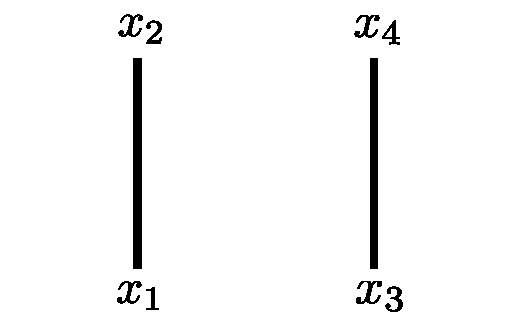
\includegraphics[scale=0.45, valign=c]{figs/diagrams/correlations/disconnected_01} \hspace{-1em}+\hspace{-1em} 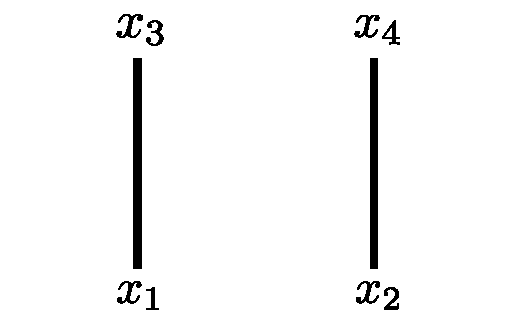
\includegraphics[scale=0.45, valign=c]{figs/diagrams/correlations/disconnected_02} \hspace{-1em}+\hspace{-1em} 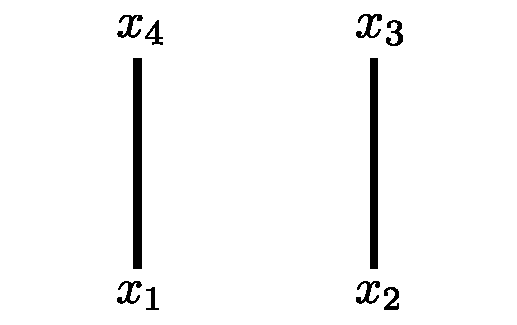
\includegraphics[scale=0.45, valign=c]{figs/diagrams/correlations/disconnected_03}
	\end{align*}
\caption[Visualization of the connected and disconnected parts contributing to the 4-point function in scalar theory.]{Visualization of the connected and disconnected parts contributing to the 4-point function in scalar theory \cite{QFTNotesFloerchingerWetterich}. The relevant contribution to the scattering process is already contained in the connected diagram.}
\label{fig:connected_correlators}
\end{figure}

From an axiomatic viewpoint, the Whightman reconstruction theorem tells us, that the complete set of corresponding $n$-point correlation functions defines the respective quantum field theory entirely and uniquely \cite{Wightman1956}. This explains why the computation of the correlation functions is a task of major importance for the theoretical understanding of a certain QFT. \\
Nevertheless, the correlation functions derived as above contain redundant information, cf. \figref{fig:connected_correlators}. For a more efficient description of the theory in terms of only the \textit{connected} correlation functions, we define the \textit{Schwinger functional} $W[J]$ as the logarithm of $Z[J]$,  
\begin{align}
W[J] = \ln Z[J].
\label{eqn:Schwinger}
\end{align}
It is the generating functional for the connected correlation functions. The normalization factor $\mathcal{N}$, introduced in \eqref{eqn:partition} enters here as an additive constant, which drops out for all higher order correlation functions, except for the 0-point function. This term is connected to the thermodynamic quantities of the system and becomes important, when external parameters such as temperature, volume or the chemical potential are tuned. Nevertheless, in general we are only interested in correlation functions with $n\geq 1$ and therefore we will not focus on this term explicitly in the following.\\
To understand how this redefinition subtracts the disconnected parts of the correlation functions, consider for example the connected 2-point function $W^{(2)}_{ab}(x_1,x_2) = W^{(2)}_{\alpha\beta}$\footnote{To save on notation, we introduce collective indices $\alpha = (x_1,a)$ or $(q_1,a)$ in momentum space.}, correlating the field $\varphi_a$ at spacetime point $x$ with the field $\varphi_b$ at $y$,
\begin{equation}
\begin{aligned}
	W^{(2)}_{\alpha\beta} &= \frac{\delta^2W[J]}{\delta J_{\alpha}\delta J_{\beta}} = \frac{\delta}{\delta J_{\alpha}}\left(\frac{1}{Z}\frac{\delta Z}{\delta J_{\beta}}\right) = \frac{1}{Z}\left(\frac{\delta^2Z}{\delta J_{\alpha}\delta J_{\beta}}\right) - \frac{1}{Z^2}\left(\frac{\delta Z}{\delta J_{\alpha}}\right)\left(\frac{\delta Z}{\delta J_{\beta}}\right)\\[0.5em]
				&= \cf{\varphi_{\alpha}\varphi_{\beta}} - \phi_{\alpha}\phi_{\beta} = \cf{\varphi_{\alpha}\varphi_{\beta}}_{\mathrm{c}}. 
\end{aligned}
\label{eqn:G_connected}						
\end{equation}
This quantity is known as the propagator, the central object of interest in functional approaches to QFT, 
\begin{equation}
	G(x_1,x_2) := W^{(2)}(x_1,x_2).
\end{equation}
It is possible to make computations even more efficient, because $W[J]$ still contains redundant information. Connected correlation functions can be separated into so-called \textit{one-particle irreducible} (1PI) and \textit{reducible} ones. In terms of diagrams, the 1PI correlation functions are those, whose corresponding Feynman diagrams can \textit{not} be separated into two disconnected parts by cutting a single internal line, cf. \figref{fig:1PI_correlators}. If the diagram is reducible in this sense, it can be expressed by multiplying the two disconnected parts with the cut propagator. The disconnected parts are then of the same or lower loop-order and are therefore already included.\\
The generating functional for the  1PI correlation functions, the \textit{effective action} $\Gamma$, is obtained from the Schwinger functional via a Legendre transformation, 
\begin{equation}
	\Gamma[\phi]=\sup _{J}\left\{\int_{x} J(x) \phi(x)-W[J]\right\}=\int_{x} J_{\mathrm{sup}}(x) \phi(x)-W\left[J_{\mathrm{sup}}\right],
\label{eqn:Def_Gamma}
\end{equation}
where $J_{\mathrm{sup}}$ has to be understood as a field-dependent current $J_{\mathrm{sup}}[\phi]$. In the following, we will drop the subscript, its meaning is implicitly understood. Note, that the effective action depends on the expectation value $\phi$ instead of the full fluctuating fields $\varphi$.

\begin{figure}[t]
\centering
\hfill
\begin{subfigure}{0.4\textwidth}
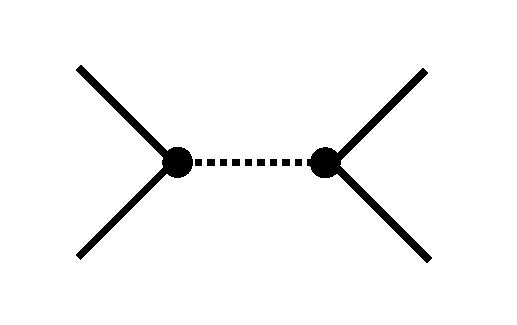
\includegraphics[scale=0.55, valign=c]{figs/diagrams/correlations/connected_02} 
\end{subfigure}
\hfill
\begin{subfigure}{0.4\textwidth}
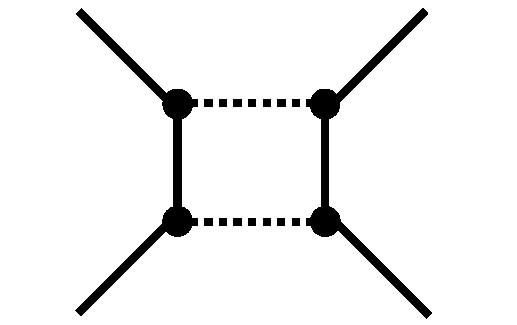
\includegraphics[scale=0.55, valign=c]{figs/diagrams/correlations/1PI} 
\end{subfigure}
\hfill

\caption[Reducible and 1PI contribution to the connected 4-point function in Yukawa theory.]{Reducible (left) and 1PI contributions (right) to the connected 4-point function in Yukawa theory \cite{QFTNotesFloerchingerWetterich}.}
\label{fig:1PI_correlators}
\end{figure}

The quantum equation of motion derived from $\Gamma$ reads
\begin{align}
	J(x) = \frac{\delta\Gamma[\phi]}{\delta\phi(x)}.
	\label{eqn:quantum_eom}
\end{align}
It allows us to understand the dynamics of field expectation values, taking the effects of all quantum fluctuations into account.
From a physical point of view, the effective action $\Gamma$ is the quantum analogue of the classical action $S$. The underlying symmetries of the classical action are in general still present in the effective action.\\
In terms of the effective action, higher order correlation functions are again obtained by performing functional derivatives, but now with respect to the mean field $\phi$,
\begin{align}
	\Gamma^{(n)}[\phi]\left(p_{1}, \ldots, p_{n}\right)=\frac{\delta^{n} \Gamma[\phi]}{\delta \phi\left(p_{1}\right) \cdots \delta \phi\left(p_{n}\right)}.
\end{align}
Here we presented the momentum space expression. The field-dependent propagator derived from the effective action is now given by the \textit{inverse} of the 1PI 2-point function:
\begin{equation}
	G[\phi](p,q) = \frac{1}{\Gamma^{(2)}}[\phi](p,q).
\end{equation}
The path integral measure of the generating functional is invariant under field independent spacetime translations $\phi(x) \rightarrow \phi(x) + \Lambda(x)$ and so are the respective correlation functions. The corresponding symmetry identity derived from this is given by
\begin{equation}
\frac{\delta \Gamma[\phi]}{\delta \phi(x)}=\frac{\delta S[\phi]}{\delta \varphi(x)}\left[\varphi=G \cdot \frac{\delta}{\delta \phi}+\phi\right]. \label{eqn:DSE}
\end{equation}
\begin{figure}[t]
\centering
\begin{subfigure}{0.3\textwidth}
	\begin{align*}
G \hspace{0.5em}= 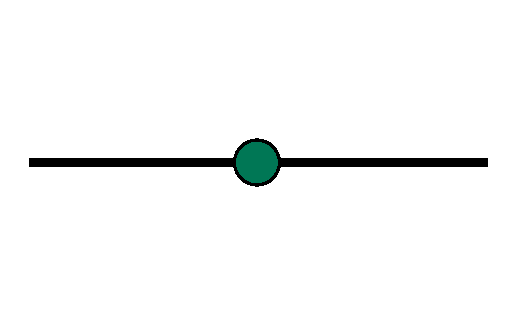
\includegraphics[scale=0.4, valign=c]{figs/diagrams/notation/full_propagator}
	\end{align*}
	\subcaption{Full propagators.}
\end{subfigure}
\hfill
\begin{subfigure}{0.3\textwidth}
	\begin{align*}
S^{(n)} = \hspace{-0.5em}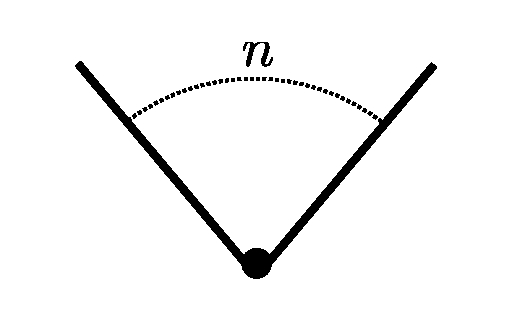
\includegraphics[scale=0.4, valign=c]{figs/diagrams/notation/classical_vertices}
	\end{align*}
	\subcaption{Bare $n$-point vertices.}
\end{subfigure}
\hfill
\begin{subfigure}{0.3\textwidth}
	\begin{align*}
\Gamma^{(n)} = \hspace{-0.5em} 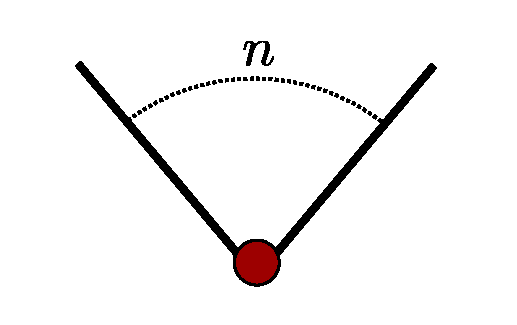
\includegraphics[scale=0.4, valign=c]{figs/diagrams/notation/full_vertices}
	\end{align*}
	\subcaption{Full $n$-point vertices.}
\end{subfigure}
\caption{Overview of the diagrammatic notation used throughout this work.}
\label{fig:notation}
\end{figure}\noindent 
This is the famous \textit{Dyson-Schwinger equation} (DSE), the central functional relation in the context of our work. The DSE therefore establishes a relation between the quantum and the classical equations of motion via the shift independence of the path integral measure. More formal derivations can for example be found in  \cite{NPgaugeLecture, AlkoferVonSmekal2000}. Here, $S[\phi]$ is the classical action of the theory at hand and
\begin{equation}
	G\cdot\frac{\delta}{\delta\phi} = \int\frac{\dd^dq}{(2\pi)^d}\ G(p,q)\frac{\delta}{\delta\phi} .
\end{equation}
This explains how we can extract the correlation functions from the DSE, i.\,e. by taking functional derivatives of equation (\ref{eqn:DSE}). The two-point function is therefore obtained by taking a single field derivative.\\
The DSE admits a diagrammatical representation in terms of full and classical propagators and vertices, respectively. The notational conventions we choose to work with throughout this thesis are displayed in \figref{fig:notation} at the beginning of the last page.\\
To give an explicit example, consider the master DSE for the scalar $\phi^4$-theory described by the action in (\ref{eqn:phi4_action}) obtained from (\ref{eqn:DSE}):
\begin{equation}
\Gamma^{(1)}[\phi]=S^{(1)}[\phi]+\frac{\lambda_{4}}{2!}\ G \cdot \phi-\frac{\lambda_{4}}{3 !}\ G \cdot\left(G \cdot \Gamma^{(3)} \cdot G\right),\label{eqn:masterDSE_scalar1}
\end{equation}
whose diagrammatic representation is displayed in \figref{fig:masterDSE_scalar}.
\begin{figure}[t]
	\centering
	\begin{align*}
	\hspace{-25 pt} 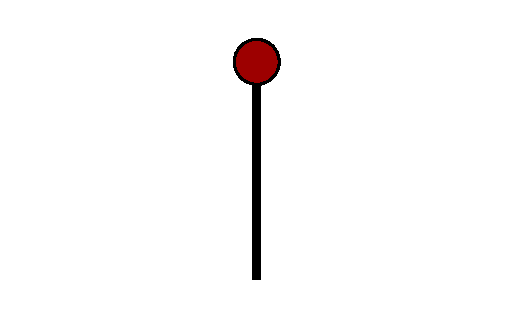
\includegraphics[scale=0.5, valign=c]{figs/diagrams/masterDSE/d_gamma} \hspace{-30 pt}=\hspace{-30 pt} 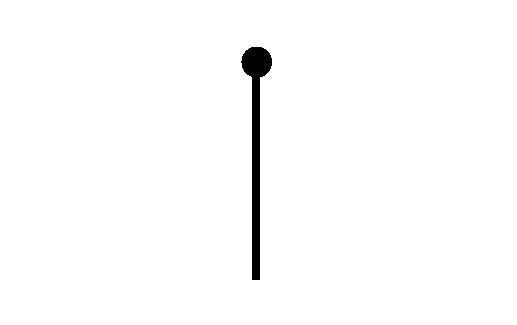
\includegraphics[scale=0.5, valign=c]{figs/diagrams/masterDSE/d_S} \hspace{-30 pt}+\hspace{20pt}\mathlarger{\frac{1}{2}} \hspace{-20 pt}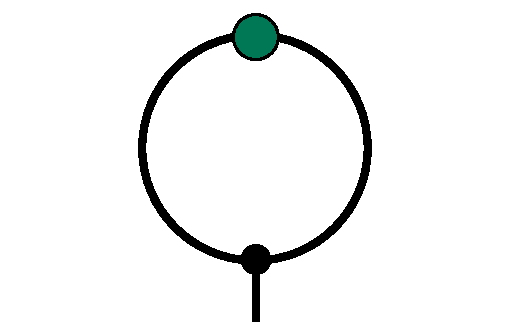
\includegraphics[scale=0.5, valign=c]{figs/diagrams/masterDSE/one_loop} \hspace{-20 pt}-\hspace{20pt} \mathlarger{\frac{1}{6}} \hspace{-20 pt}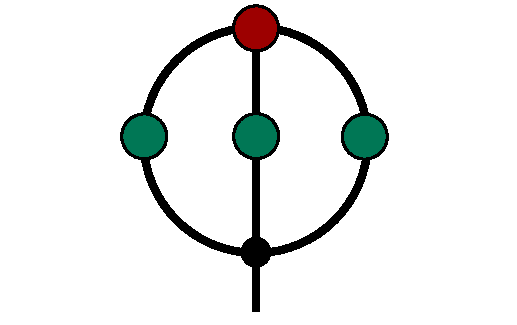
\includegraphics[scale=0.5, valign=c]{figs/diagrams/masterDSE/two_loop}
	\end{align*}
	\caption{Diagrammatic representation of the master DSE in scalar theory (\ref{eqn:masterDSE_scalar1}).}\label{fig:masterDSE_scalar}
\end{figure}

\section{K\"all\'{e}n-Lehmann Spectral Representation}
When applying functional methods such as the DSE in non-perturbative calculations involving loop corrections, the \enquote{classical} momentum scaling
\begin{equation}
	G(p)\sim\left(p^2+m^2\right)^{-1},
\end{equation}
of the propagators for some (possibly vanishing) mass scale $m$ is usually modified. This subtlety can cause severe complications in analytical and numerical computations. A rather simple approach to circumvent this  is provided by the K\"all\'{e}n-Lehmann (KL)  spectral representation \cite{Kallen1952, Lehmann1954} of the propagator, which can be derived from a completeness relation for zero momentum states of the theory, cf. \cite{QFTNotesPawlowskiJaeckel} for a detailed derivation.\\
 The KL representation allows us to recast the propagator in terms of a spectral integral over the respective spectral density (or spectral function) $\rho(\lambda^2)$ with spectral parameter $\lambda$ as follows:
\begin{align} 
G(p)=\int_{0}^{\infty} \frac{\dd \lambda^2}{\pi} \frac{\rho(\lambda^2)}{p^{2}+\lambda^{2}}. \label{eqn:KL_rep}
\end{align}
This can be interpreted as an integral over classical free propagators of a particle with squared mass $\lambda^2$ weighted by the spectral density $\rho(\lambda)$, or for the case of asymptotic states, as probability density for the transition to an excited state with energy $\lambda$. The spectral density $\rho(\lambda)$ encodes all the information about the energy spectrum of the theory.\\
The existence of a spectral representation has been discussed for decades in axiomatic approaches to QFT, cf. \cite{Wightman1965}. This poses strong conditions on the analytic structure of the propagator and imposes tight restrictions on its functional space.\\ Throughout this work, we implicitly assume its existence and in addition a cross-check to benchmark our results is always given by the comparison of the analytical result for the Euclidean propagator with the result from \eqref{eqn:KL_rep} for the computed spectral function. \\
Concerning a mathematical interpretation, the spectral function arises as the set of non-analyticities of the propagator, whose locations in the complex plane are restricted by Cauchy's theorem, cf. \figref{fig:cauchy}.\\
\begin{figure}[t]
	\centering
	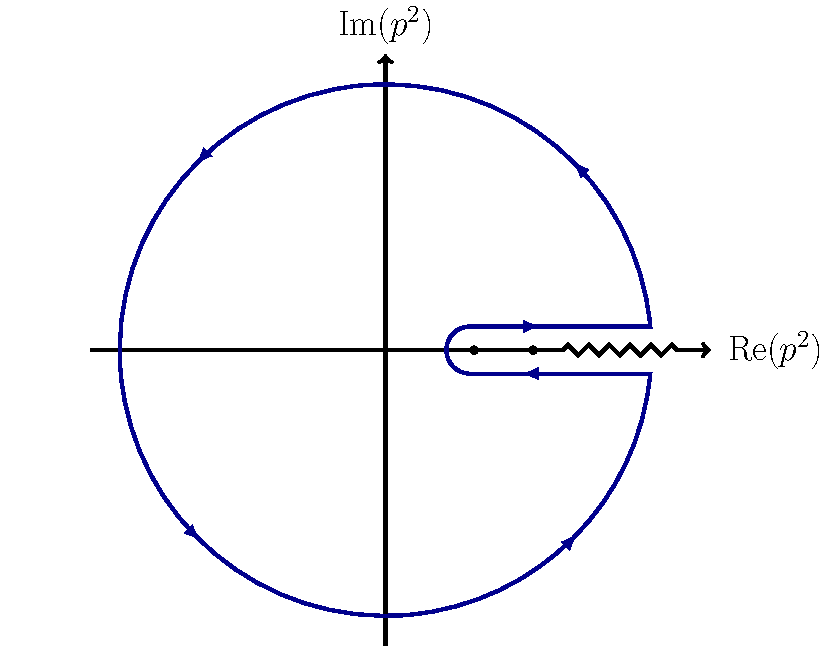
\includegraphics[width=0.6\textwidth]{figs/tikz/contour}
	\caption[Illustration of the analytic structure of an example propagator for a scalar theory featuring a 2-particle bound-state.]{Illustration of the analytic structure of an example propagator for a scalar theory featuring a 2-particle bound-state. The contour is chosen in such a way that all the non-analyticities of the propagator are excluded and corresponds to the evaluation of \eqref{eqn:KL_rep} using Cauchy's theorem. The visualization is inspired by \cite{JiaPennington2017}.} 
	\label{fig:cauchy}
\end{figure}\noindent
From this, an inverse relation between the retarded propagator and the spectral function can be derived, cf. \appref{chap:appendixB} for a detailed derivation. It reads
\begin{equation}
	\rho(\omega, \abs{\mathbf{p}}) = 2 \operatorname{Im}\left[G\left(-i(\omega + i0^+), \abs{\mathbf{p}}\right)\right], \label{eqn:specfunc_relation}
\end{equation}
with $\omega$ being the zero component of the real-time momentum and $0^+$ has to be understood as taking the limit $\varepsilon\rightarrow 0$ from above. This relation is of particular importance, since we will use it later on to extract the spectral function from the computed retarded propagator.\\
 Note, that in this instance, the spectral function is expressed as a function of a linear argument in contrast to the definition in \eqref{eqn:KL_rep}, which is the convention we choose to work with for the remainder of this work. Imposing Lorentz invariance usually enforces the propagator to be a function of $p^2$ and therefore the same must hold for the spectral function. Nevertheless, symmetry arguments for the analytic structure of the propagator in the complex plane allow for a change of variables $\dd\lambda^2 \rightarrow \lambda\ \dd\lambda$.\\
Following the same line of arguments, we do not need to consider the spatial momentum dependence explicitly since for vacuum QFTs all kinematic information can be restored from Lorentz transformations. Hence, we will drop the explicit dependency for the remainder of this work.  \\ 
\begin{figure}[t]
\centering
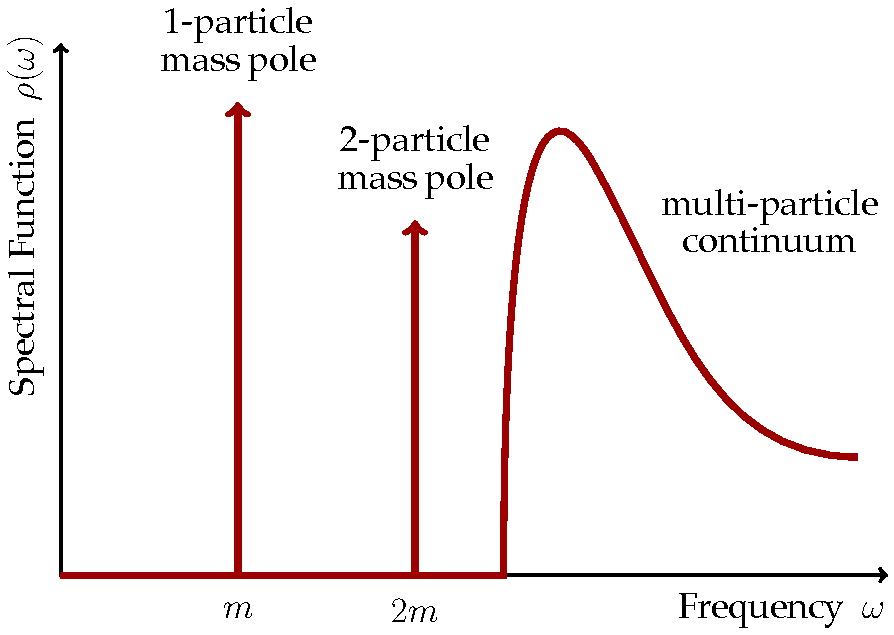
\includegraphics[width=0.6\textwidth]{figs/tikz/scalar_spec_func}
\caption[Shape of a typical spectral function of a scalar theory.]{Shape of a typical spectral function of a scalar theory. The isolated poles of the propagator show up as delta peaks in the spectral function. The continuous tail is generated by branch cuts. The visualization is inspired by \cite{Horak2019}.}\label{fig:scalar_spec_func}
\end{figure}\noindent
From equations (\ref{eqn:KL_rep}) and (\ref{eqn:specfunc_relation}) it follows straightforwardly, that all non-analycities of the propagator are restricted to the real momentum axis. This allows us to split the spectral function into pole contributions and a continuous (scattering) part generated by branch cuts, i.\,e.
\begin{equation}
	\rho(\lambda) =\sum\limits_{i} \frac{\pi R_i}{2\lambda}\ \delta(\lambda-m_i) + \rho_{\mathrm{cont}}(\lambda). \label{eqn:split}
\end{equation}
Here, the $R_i$ are the residues associated to the respective poles at $m_i$.
From this ansatz, the spectral function reproducing the classical propagator is simply obtained from equation (\ref{eqn:split}) by setting $R_1 = 1$, $R_{i>1} = 0 $ and $\rho_{\mathrm{cont}}=0$. An examplary spectral function in the context of a scalar theory is visualized in \figref{fig:scalar_spec_func}.\\
Concerning its probabilistic interpretation, one would expect the spectral density to be positive semi-definite, and for the case of scalar theory considered here, this is indeed true. The following summation rule holds:
\begin{equation}
	\int_0^{\infty}\frac{\dd\lambda}{\pi} \lambda\rho(\lambda) = 1.
\end{equation}
This picture might change for gauge theories, and especially for QCD, since the spectral functions we are interested in, are not spectral functions of asymptotic states and hence not observables. Nevertheless, it is expected that \eqref{eqn:specfunc_relation} is still true. Specifically for QCD, there exists a so-called superconvergence relation \,
\begin{equation}
	\int_0^{\infty}\frac{\dd\lambda}{\pi} \lambda\rho_A(\lambda) = 0.
\end{equation}
This relation makes positivity violation even necessary! On the technical side, a frequently occurring problem is the observation of (possibly) existing complex-conjugated poles, which would be in contradiction with the assumptions made by axiomatic QFT as discussed before.  For further details, cf. \cite{Lowdon2015}. \\
To conclude this section we again want to emphasize that working with spectral representations can facilitate computations a lot, allows for the application of perturbative techniques and can be easily implemented in calculations, as we will see later. Following the recent progress in the pure gauge sector of QCD, we want to dedicate this work to the study of the spectral properties of the matter sector of QCD, which in the end might be the key to access and predict macroscopic observables of QCD such as bulk and shear viscosities.



